\documentclass[
%draft,				% Entwurf --> Endversion mit final
dvips,
twoside,			% Doppelseiteiger Druck 
a4paper, 			% Papierformat: DIN-A4
12pt, 				% Standardschriftgroesse
headsepline, 		% Trennlinie unter Kopfzeile
plainheadsepline,	% Trennlinie auch auf Seiten mit Stil 'plain' (z. B. Kapitelanfaenge)
% footsepline, 		% Trennlinie ueber Fusszeile
% cleardoubleempty, 	% keine Kopf und Fusszeilen bei leeren Seiten
titlepage,			% Dokument mit Titelseite
BCOR1cm,			% Bindekorrektur
bibliography=totoc,			% Literaturverzeichnis im Inhaltsverzeichnis
index=totoc,
listof=totoc,
%openany,			% Kapitel koennen auch auf linker Seite beginnen
%chapterprefix,		% Vor der Kapitelueberschrift wird "Kapitel" eingefuegt
numbers=noenddot,	% Keine Punkte hinter der Kapitelnummer
appendixprefix,		% Vor den Anhangkapiteln wird "Anhang" eingefuegt
headings=small,		% Ueberschriftengroesse (smallheadings --> kleine Ueberschriften)
toc=listof
]
{scrbook}

%% Put your information in the {...} in the following commands
\newcommand{\name}{Vorname Nachname} 
\newcommand{\studenttitle}{Herr} % oder Frau
\newcommand{\regnumber}{SA/DA 20xx / XX}
\newcommand{\docType}{Diplomarbeit}
\newcommand{\docTitle}{Titel der Arbeit}
\newcommand{\abgabemonat}{Monat Jahr}
\newcommand{\abgabedatum}{Tag.Monat.Jahr}
\newcommand{\anfangsdatum}{Tag.Monat.Jahr}
\newcommand{\university}{University ...}
\newcommand{\institut}{Institut for ...}
\newcommand{\fachgebiet}{Fachgebiet ...}
\newcommand{\professor}{Prof. Dr.-Ing. Vorname Nachname}
\newcommand{\betreuer}{Dipl.-Ing. Vorname Nachname}

% Template-style
\usepackage{emt}

\usepackage[textwidth=1.5cm, textsize = tiny, color = red, dvistyle, ngerman, colorinlistoftodos]{todonotes}	% Entfernen mit [disable]

% Declare own mathematical operators
\DeclareMathOperator{\grad}{grad}	% Normale mathematische Funktion
\DeclareMathOperator{\DIV}{div}
\DeclareMathOperator{\rot}{rot}
\renewcommand{\j}{\mathrm{j}}

% Declare shortform for 'difficult' names
\newcommand{\matlab}{$\textnormal{\textsc{Matlab}}^{\scriptstyle \circledR} $ } 

% Declare hyphenation for single words, that are not known by the dictionary or where you wish a different hyphenation
\hyphenation{
Grafik-karten-pro-zes-sor % example. Please add your own
}

% Image-folder
\graphicspath{{img/}}

% PSTricks Makros
\newcommand*\pswall[3]{ % Produces the symbol for a wall
	\psframe[linecolor=white,fillstyle=hlines,hatchcolor=black](#1)(#2)
	\psline[linecolor=black](#1)(#3)}


%% Start of document
\begin{document}
\SIunits[mediumqspace,mediumspace] % Set options for SIunits-packet

\frontmatter

% Titelseite
\thispagestyle{empty}

\begin{titlepage}
	{
		\begin{flushleft}
				\hspace{10mm}\textbf{\institut}\\
				\hspace{10mm}\university\\
				\hspace{10mm}\fachgebiet\\
				\hspace{10mm}\professor
		\end{flushleft}

		\begin{picture}(0,0)(0, -22.5)
			\put(-35,5){\includegraphics[height=20mm]{uni-logo.eps}}
			\put(310,5){\includegraphics[height=20mm]{fg-logo.eps}}
		\end{picture}
	}

	\begin{center}
		\vspace{10mm}
		{\bfseries \large \docType}

		\vspace{25mm}
		{\bfseries \LARGE \docTitle}

		\vspace{25mm}
		{\large von \\[3mm]}
		{\Large \name}\\[3mm]
		{\itshape (Registriernummer: \regnumber)}

		\vspace{15mm}
		{\large
		\begin{tabular}{l l}
			Betreuer: 	& \professor \\
									& \betreuer \\
		\end{tabular}}

		\vspace{15mm}
		{\large Paderborn im \abgabemonat }

	\end{center}
\end{titlepage}


% Zweite Titelseite
\begin{titlepage}
	{
		\begin{flushleft}
				\hspace{10mm}\textbf{\institut}\\
				\hspace{10mm}\university\\
				\hspace{10mm}\fachgebiet\\
				\hspace{10mm}\professor
		\end{flushleft}

		\begin{picture}(0,0)(0, -22.5)
			\put(-35,5){\includegraphics[height=20mm]{uni-logo.eps}}
			\put(310,5){\includegraphics[height=20mm]{fg-logo.eps}}
		\end{picture}
	}

	\vspace{5mm}
	\begin{flushright}
		Nr. \regnumber
	\end{flushright}

	\vspace{15mm}
	\begin{center}
		\large
		\docType \\[4mm] f�r \\[4mm]
		\studenttitle \; \name \\
	\end{center}

	\vspace{15mm}
	\begin{flushleft}
		Thema: \docTitle			\\[30mm]
		\professor 	\\[15mm]
		Datum der Ausgabe: \anfangsdatum	\\[10mm]
		Datum der Abgabe: \abgabedatum
	\end{flushleft}
\end{titlepage}
\setcounter{page}{1} % set page-counter to one

% Declaration of own work (may be dropped for some thesis)
\newpage
\chapter*{Erkl�rung}

Ich versichere, die Arbeit selbstst�ndig angefertigt, 
alle benutzten Hilfsmittel vollst�ndig und genau angegeben 
und kenntlich gemacht zu haben, was aus Arbeiten anderer 
unver�ndert oder mit Ab�nderungen entnommen wurde.

\begin{tabbing}
Paderborn, den \hspace{0.4cm} \= \rule[-0.15\baselineskip]{5cm}{.4pt}  \hspace{0.7cm}\= \rule[-0.15\baselineskip]{6cm}{.4pt}\\
\renewcommand{\baselinestretch}{0.5}\normalsize
\>\small{(Datum)}\>\small{(Unterschrift)}
\end{tabbing}
\cleardoublepage

\listoftodos		% Show todo-list here

\maintoc				% table of contence
\listoffigures	% list of figures
\listoftables		% list of tables

\addchap{Verzeichnis der verwendeten Abk�rzungen und Symbole}
\section*{Verwendete Abk�rzungen}
\begin{longtable}[l]{p{4cm} p{10cm}}\toprule
		\textbf{Abk�rzung} 		& \textbf{Bedeutung} \\ 
		\midrule \endhead
		\bottomrule \endfoot
	FEM						& \emph Finite \emph Element \emph Methode\\
	IEEE					& Institute of Electrical and Electronics Engineers \\
	$\nabla \left\{\cdot\right\}, \grad \left\{\cdot\right\}$ 		& Gradientenoperator \\
	$\nabla^2\left\{ \cdot \right\} , \Delta\left\{ \cdot \right\}$		& Laplaceoperator \\
\end{longtable}

\section*{Verwendete Formelbuchstaben}
\begin{longtable}[l]{p{3cm} p{2cm} p{9cm}} \toprule
		\textbf{Formelzeichen} & \textbf{Einheit} & \textbf{Bedeutung} \\ \midrule \endhead
		\bottomrule \endfoot
		$\vec{E}$			& \unit{}{\volt\per\meter}		& Elektrische Feldst�rke\\
		$\vec{p}$			& 						& Schallwechseldruck \\
		$\psi$				& 						& Akustisches skalares Potential \\
	\end{longtable}
\cleardoublepage

\addchap{Kurzfassung}
	\label{cha:Kurzfassung}


\todo[inline]{Kurzfassung (ca. 100 W�rter)}



\mainmatter
\chapter{Kurze Einf�hrung in \LaTeX}
\label{chapter:introduction}

In diesem Kapitel \ref{chapter:introduction} werden die wichtigsten LaTeX-Konstrukte kurz vorgestellt. Es empfielt sich, das PDF-Dokument mit dem \LaTeX - Quelltext zu vergleichen, um die Syntax zu erlernen. Viele Quelltextbl�cke aus diesem Dokument k�nnen einfach in eingene Dokumente kopiert werden und ben�tigen dann nur noch geringe Anpassungen, so z.B. zum Einbinden von Grafiken, was in Abschnitt \ref{section:figures} vorgestellt wird.

\section{Formeln}
\label{section:equations}

Dieser Abschnitt befa�t sich mit der Verwendung von Formeln.
Das PDF-Dokument \textit{short-math-guide.pdf} ist eine gute Anlaufstelle bei Fragen und Problemen (siehe Ordner: \textsc{lesenswertes}).

\subsection{Inline-Formeln}
\label{subsection:inlineEquation}

Inline-Formeln stehen mittem im Textfluss. Dazu wird die Formel durch \$-Zeichen im Quelltext eingerahmt. Beim �bersetzen des Dokumentes wird dann die sch�n gerenderte Formel erzeugt. Hier ein Beispiel: $e^x = \sum\limits_{n=0}^{\infty}\frac{x^n}{n!}$

\subsection{Die equation-Umgebung}
\label{subsection:defaultEquation}

Die im vorherigen Abschnitt \ref{subsection:inlineEquation} eingef�hrte Formel schreibt sich mit Hilfe der \textit{equation}-Umgebung wie folgt:
\begin{equation}
\label{equation:expFunktion}
 e^x = \sum\limits_{n=0}^{\infty}\frac{x^n}{n!}
\end{equation}
Hinweis: \textit{eqref} fa�t die Nummer der Gleichung automatisch in runde Klammern, so dass beim Referenzieren auf Gleichungen die Klammern nicht aus versehen vergessen werden k�nnen.

\section{Literaturquellen referenzieren}
\label{section:literaturref}
Die Literaturquellen werden mit Hilfe von \textsc{bibtex} referenziert. Die Quellen k�nnen in unterschiedlichen  ''.bib'' Dateien beschrieben sein (siehe z.B. \url{bibs/ruoff.bib}). Der Aufruf im Dokument erfolgt dann gem��:
\begin{verbatim}
	\bibliographystyle{IEEEtran}
	\bibliography{IEEEfull,bibs/ruoff,bibs/weitere_bib}
\end{verbatim}
Die Form der Abk�rzungen steht in \url{bibs/IEEEfull.bib}, welche vor allen Bibliotheken eingebunden wird. Alle referenzierten  Quellen werden automatisch in das Literaturverzeichnis eingf�gt, ein Fehler erscheint, wenn der \\cite\{\}-Befehl nicht verwendet wurde.

Eine Quelle aus einer Datenbank wird so referenziert: \textbackslash cite\{bibtexkey\} und sieht dann so aus: \cite{DudaHartStork01}


\section{Tabellen}
\label{A}

Dieser Abschnitt \ref{A} befa�t sich mit der Verwendung von Tabellen. Tabellen haben, im Gegensatz zu Grafiken, eine �berschrift, keine Unterschrift. In der Regel werden in Tabellen keine vertikalen Linien verwendet, horizontale Linien nur vor und nach �berschrift und Fu�zeile, was aber durch die Verwendung von \texttt{\textbackslash toprule}, \texttt{\textbackslash midrule} und \texttt{\textbackslash bottomrule} automatisch eingef�gt wird. Handelt es sich um eine lange Tabelle, die �ber mehrere Seiten umgebrochen werden kann, so kann der Typ \texttt{longtable} verwendet werden (siehe \texttt{frontmatter/Verzeichnisse.tex}), bei dem die Kopfzeile automatisch auf jeder Seite wiederholt wird.
\begin{table}[hbt!]
	\caption{Eine einfache Tabelle}
  \begin{center}
    \begin{tabular}{clr}
      \toprule
      \bf laufende & \bf Wert 1 & \bf Wert 2\\
      \bf Nummer  & & \\
      \midrule
      $1$ &  $1\,000$ & $20$  \\
      $2$ &  $1\,500$ & $40$  \\
      \bottomrule
    \end{tabular}
  \end{center}
\label{tab:table_1}
\end{table}

 \section{Listen und Aufz�hlungen}
Listenumgebungen werden durch \texttt{\textbackslash begin\{itemize\}} eingeleitet. \texttt{\textbackslash end\{itemize\}} beendet die Umgebung. Jedem Eintrag wird ein \texttt{\textbackslash item} vorgestellt.
Soll die Liste nummeriert werden, wird statt \textit{itemize} die \textit{enumerate}-Umgebung benutzt. F�r Definitionslisten wird die \textit{description}-Umgebung verwendet.

Das Ergebnis sieht dann so aus, wie in den folgenden beiden Beispielen.
 
 
\begin{enumerate}
	\item Erster Eintrag
	\item Zweiter Eintrag
	\begin{enumerate}
		\item Listen k�nnen auch mehrere Ebenen enthalten
	\end{enumerate}
	\item Dritter Eintrag	
\end{enumerate}

\begin{itemize}
	\item Liste, die
	\item keine Nummerierung
	\item enth�lt.
\end{itemize}


\section{Einheiten}
Die korrekte Darstellung der SI-Einheiten ist f�r unmissverst�ndliche Darstellungen unabdingbar. Hier hilft das  \textsc{SIunits}-Paket.

Sowohl in Mathe-Umgebungen wie auch im Flie�text werden Zahlen mit Einheit durch \texttt{\textbackslash unit\{<Wert>\}\{<Einheit(en)>}\} dargestellt. Als Einheit wird z.B. \textbackslash meter, \textbackslash ampere oder \textbackslash kelvin verwendet. Eine vollst�ndige Liste der unterst�tzten Einheiten ist in der Dokumentation zu dem Paket zu finden (Datei \textsc{SIunits.pdf} im Ordner \textsc{lesenswertes}) Die Ausgabe kann dann wie Folgt aussehen:
\begin{itemize}
	\item \unit{1,45}{\kilo\gram}
	\item \unit{477,38}{\volt\meter\per\squaren\second}
\end{itemize}

Die Eingabe der Einheiten in dieser Form erscheint zun�chst kompliziert, setzt alle Einheiten aber korrekt - n�mlich gerade, mit einem verkleinerten Abstand zwischen Ziffer und Einheit und ohne Zeilenumbruch zwischen Zahl und Einheit.

\section{Beispiele}
F�r Beispiele gibt es eine separate Umgebung, n�mlich die \texttt{example} Umgebung.
\begin{example}
	Nummeriertes Beispiel ...
	\label{exa:bsp_test}
\end{example}

\section{Grafiken}
\label{section:figures}
Zum Einbinden von Grafiken stehen in \LaTeX verschiedene M�glichkeiten zur Verf�gung.

Diese Vorlage geht davon aus, dass das Dokument NICHT mit \textit{pdflatex} sondern mit reinem \textit{latex}. Daher werden nur Vektorgrafikformate (.eps, .ps, .bmp, .pict) akzeptiert. Wird pdfLaTeX genutzt, k�nnen NUR Grafikdateien in den Formaten .jpeg, .png und .pdf genutzt werden. Das �bersetzen dieses Dokumentes wird daher voraussichtlich fehlschlagen.

\subsection{EPS mit Textersetzungen (psfrag)}
Dieser Abschnitt stellt kurz das Einf�gen von Grafiken und das Ersetzen von Text innerhalb einer eps-Datei durch LaTeX-eigene Schriften und insbesonder auch Formeln vor. 

Die Verwendung des \textit{PSfrag}-Packets wird in der \textit{psfrag-guide.pdf} Datei n�her erkl�rt (siehe Ordner: \textsc{lesenswertes}).

ACHTUNG: Die Ersetzungen sind erst in der PS/PDF-Datei an der gew�nschten Stelle. In der DVI-Datei sind die Ersetzungen nur aufgelistet.
\begin{figure}[!ht]
	\centering
	\psfragscanon
	\psfrag{Sinuskurve}[][c]{$u(\varphi) = 1 \mathrm{V} \cdot \sin(\varphi)$}
	\psfrag{phi / rad}[][r]{\large $\frac{\varphi}{\mathrm{rad}}$}
	\psfrag{u / V}[][c][1][-90]{\large $\frac{u}{\mathrm{V}}$}
	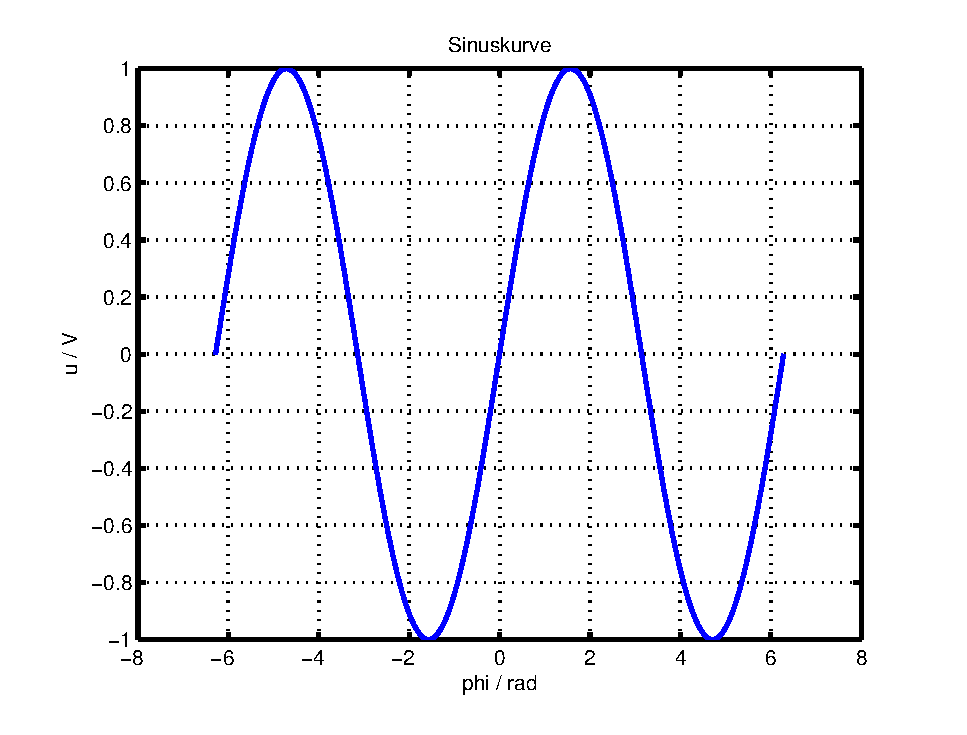
\includegraphics[width=0.8\textwidth]{sinus.eps}
	\psfragscanoff
	\caption{Sinusf�rmiger Spannungsverlauf}
	\label{fig:sin}
\end{figure}
\clearpage

\subsection{PS-Tricks}
Mit PS-Tricks lassen sich Grafiken direkt im \LaTeX - Code 'malen'. Die beiden Folgenden Grafiken sind komplett mit PS-Tricks erstellt.
\begin{figure}[htb!]
	\centering
	
\begin{pspicture}[showgrid=false](8,5)
	\pnode(0,0){A}
	\pnode(4,0){B}
	\pnode(0,4){C}
	\pnode(4,4){D}
	\pnode(8,4){E}
	\pnode(8,0){F}
	\resistor(C)(D){$R_{v_1}$}
	\resistor(D)(E){$R_L$}
	\LED(E)(F){$D_L$}
	\Zener[labeloffset=-0.7](B)(D){$D_Z$}
	\Ucc(A)(C){$U$}
	\wire(A)(C)
	\wire(A)(B)
	\wire(F)(B)
\end{pspicture}
		\caption{Test mit PST-circ}
\end{figure}


\begin{figure}[h!]
\centering
	\begin{pspicture}(-2,-4)(2,4)
	\pswall{-2,2.5}{2,3.5}{2,2.5}
	\pnode(-1,1.5){A}
	\pnode(-1,-1.5){B}
	\pnode(1,1.5){C}
	\pnode(0,-1.5){D}
	\pnode(1,-1.5){E}
	\pnode(0,-4){F}
	
	\cnode[fillstyle=solid,fillcolor=lightgray](0,-2.5){0.5}{Mass}
	\rput[c](Mass){$m$}
	
	\psline{-}(A)(C)
	\psline{-}(D)(B)
	\psline{-}(D)(E)
	\ncline{D}{Mass}
	\psline{-}(0,1.5)(0,2.5)
	
	\psline[linewidth=2pt]{-}(1.6, -2.5)(2.4, -2.5)
	\pnode(2,-2.5){Us}
	\pnode(2,-4){Ue}
	\ncline[arrows=|->, arrowsize=4pt]{Us}{Ue}
	\ncput{\hspace{10mm}$u(t)$}
	\ncline[arrows=->, arrowsize=4pt]{Mass}{F}
	\ncput{\hspace{10mm}$f(t)$}
	\resistor[dipolestyle=zigzag](B)(A){$k$}% spring
	\dashpot(E)(C){$d$}% dashpot
	\end{pspicture}
	\caption{Ged�mpfter Einmassenschwinger}
	\label{fig:Einmassenschwinger}	
\end{figure}


\subsection{\texorpdfstring{\matlab}{Matlab} Plots}
Zur Darstellung von Kurven (z.B. Simulationsergebnisse, Messergebnisse), die mit \matlab generiert wurden, k�nnen direkt \matlab-dat-Dateien in Latex eingelesen werden und die Achsen und Beschriftungen von Hand im \LaTeX-Quelltext erg�nzt werden.

\begin{figure}[!ht]
	\centering
	\psset{axesstyle = axes, xAxisLabel = $ \frac{f}{ \mathrm{Hz}}$, yAxisLabel = $ {\alpha , \beta } $}
	\begin{psgraph}[arrows = ->, arrowscale=3, ticks = none, subticks = 4, Dx=10 , Dy =25 ](0,0)(0,0)(55,75){10cm}{5cm}
	\readdata{\rayleigh}{img/alpha.dat}
	\dataplot[plotstyle=curve,showpoints=false,linecolor=blue, linewidth=1.5pt]{\rayleigh}
	\readdata{\rayleigh}{img/beta.dat}
	\dataplot[plotstyle=curve,showpoints=false,linecolor=red, linewidth=1.5pt]{\rayleigh}
	\rput(54,60){$\beta \sim f$}
	\rput(5,45){$\alpha \sim \frac{1}{f}$}
	\end{psgraph}
	\caption{Rayleighd�mpfungsparameter $\alpha$ und $\beta$}
	\label{fig:Rayleigh}	
\end{figure}


% add your chapters here


%%%%%%%%%%%%%%%%%%%%
% this is where the backmatter starts
%\backmatter % toggling this comment results in chapter names with or without capital numbering
% the bibliography
%\addcontentsline{toc}{chapter}{Literaturverzeichnis}
% the bibliography shouldn't have a consecutive numbering
\ihead{\leftmark}
\bibliographystyle{alphadin} 		% alphabetical order ([Abc09]) 
%\bibliographystyle{unsrtdin}		% Sortierung nach Reihenfolge der Zitate im Dokument ([1], ...) 
\bibliography{bibs/IEEEfull,bibs/ruoff}
\clearpage
% but the appendix could
\ihead{\thechapter~\leftmark}
% the appendix is part of the backmatter, but uses capital numbering by default


% Appendix
% \pagenumbering{alph}
\setpartpreamble[u,r][8cm]{\vspace{20mm}Erweiterte Informationen zu der vorliegenden Arbeit}\part*{Anhang}
\appendixtoc
\appendix

\chapter{...}




\addchap{Inhalt der Begleit-CD}
\begin{enumerate}
	\item 	
	\item	Elektronisch verf�gbare Literaturquellen
\end{enumerate}


\end{document}
%% End of document
